%% LyX 2.2.2 created this file.  For more info, see http://www.lyx.org/.
%% Do not edit unless you really know what you are doing.
%\documentclass[english,conference,onecolumn]{IEEEtran}
\documentclass[english]{article}
\usepackage{spconf}
\usepackage{array}
\usepackage[T1]{fontenc}
\usepackage[utf8]{inputenc}
\usepackage{geometry}
\usepackage{algorithmic}
\usepackage{varwidth}
\usepackage{listings}
\geometry{verbose,tmargin=2cm,bmargin=2cm,lmargin=2cm,rmargin=2cm}
\usepackage{amsmath}
\usepackage{graphicx}
\usepackage{float}
\usepackage{babel}
\newfloat{algorithm}{tbp}{loa}
\floatname{algorithm}{Algorithm}

%\ninept\name{Jean-Marc Valin, Steinar Midtskogen}\address{Mozilla Corporation\\Mountain View, CA, USA}
\ninept
\twoauthors
{Jean-Marc Valin}{Mozilla Corporation\\Mountain View, CA, USA\\\texttt{jmvalin@jmvalin.ca}}
{Steinar Midtskogen}{CISCO (add more details)}

\makeatletter

\newcolumntype{C}{>{\centering\arraybackslash}p{0.8em}}
\newcolumntype{X}{>{\centering\arraybackslash}p{10.5em}}

%%%%%%%%%%%%%%%%%%%%%%%%%%%%%% LyX specific LaTeX commands.
%% Because html converters don't know tabularnewline
\providecommand{\tabularnewline}{\\}

%%%%%%%%%%%%%%%%%%%%%%%%%%%%%% User specified LaTeX commands.
\usepackage{color}
\usepackage{url}
\usepackage[pdfpagemode=None,pdfstartview=FitH,pdfview=FitH,colorlinks=true,pdftitle=The AV1 Constrained Directional Enhancement Filter,pdfauthor=Jean-Marc Valin]{hyperref}

\makeatother

\begin{document}

\title{The AV1 Constrained Directional Enhancement Filter}

\maketitle
\begin{abstract}
This paper presents the constrained directional enhancement filter
designed for the AV1 royalty-free video codec. The filter is based on
a non-linear low-pass filter and is designed for vectorization
efficiency. It takes into account the direction of edges and patterns
being filtered. The filter works by identifying the direction of each
block and then adaptively filtering with a high degree of control over
the filter strength along the direction and across it.  The proposed
enhancement or deringing filter is shown to improve the quality of the
Alliance for Open Media (AOM) AV1 video codec in particular in low
complexity configurations.
\end{abstract}

\begin{keywords}enhancement filter\end{keywords}

\section{Introduction}

The main goal of deringing is to filter out coding artifacts while
retaining the details of the image. In HEVC, this is achieved by the
Sample Adaptive Offset~(SAO)~\cite{HEVC-SAO} algorithm that defines
signal offsets for different classes of pixels. Unlike SAO, the
approach we take in AV1 is that of a non-linear spatial filter.  From
the very beginning, the design of the filter was constrained to be
easily vectorizable (i.e. implementable with SIMD operations), which
was not the case for other non-linear filters like the median
filter~\cite{Median} and the bilateral filter~\cite{Bilateral}.

The design of the deringing filter originates from the following observations.
The amount of ringing in a coded image tends to be roughly proportional
to the quantization step size. The amount of detail is a property
of the input image, but the smallest detail actually retained in the
quantized image tends to also be proportional to the quantization
step size. For a given quantization step size, the amplitude of the
ringing is generally less than the amplitude of the details.

This paper describes the constrained directional enhancement filter
(CDEF), a deringing filter that takes into account the direction of
edges and patterns being filtered. CDEF works by identifying the
direction of each block and then adaptively filtering along the
identified direction and also to a lesser degree along directions 45
degrees off the identified direction.  The filter strength along the
direction and 45 degrees off it can be signalled separately, which
allows a high degree of control over the blurring.

\section{Direction Search}

The proposed deringing filter is based on the direction of edges,
so we will start by describing the direction search. For this, the
image is first divided into blocks of $8\times8$. The block size
is chosen to be fine enough to adequately handle non-straight edges,
while being large enough to reliably estimate directions when applied
to a quantized image. Having a constant direction over an $8\times8$
region also makes vectorization of the filter easier.

For each block we want to determine the direction that best matches
the pattern in the block. This is done by minimizing the sum of squared
differences (SSD) between the quantized block and a perfectly directional
block. A perfectly directional block is a block for which each line
along a certain direction has a constant value. For each direction,
we assign a line number $k$ to each pixel, as shown in Fig.~\ref{fig:Lines-for-direction}. 

\begin{figure}
\centering{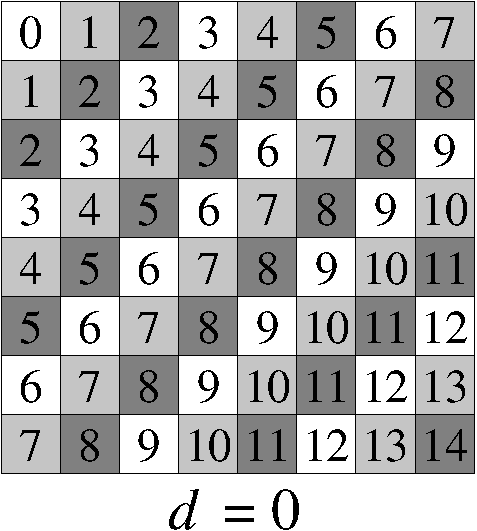
\includegraphics[width=0.23\columnwidth]{dlines0}\hspace{.5em}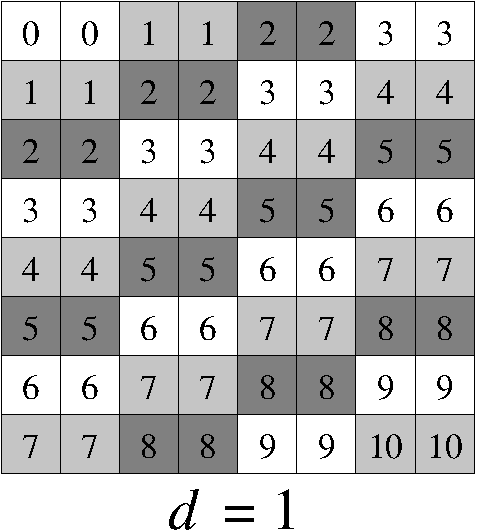
\includegraphics[width=0.23\columnwidth]{dlines1}\hspace{.5em}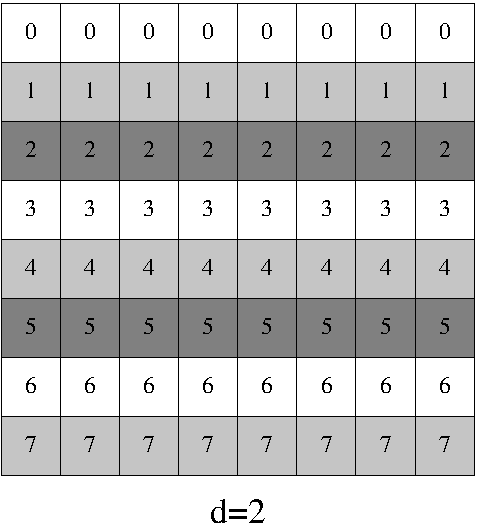
\includegraphics[width=0.23\columnwidth]{dlines2}\hspace{.5em}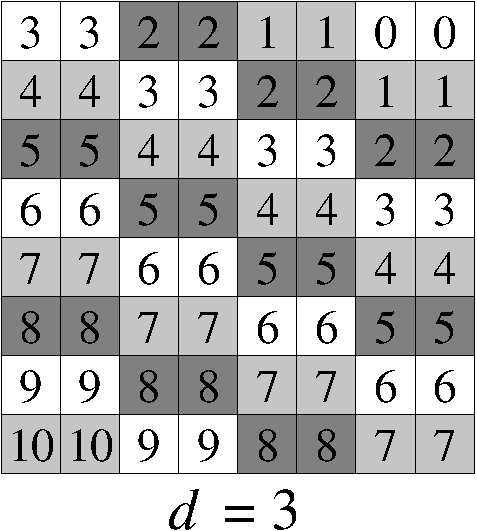
\includegraphics[width=0.23\columnwidth]{dlines3}}

\vspace{.5em}

\centering{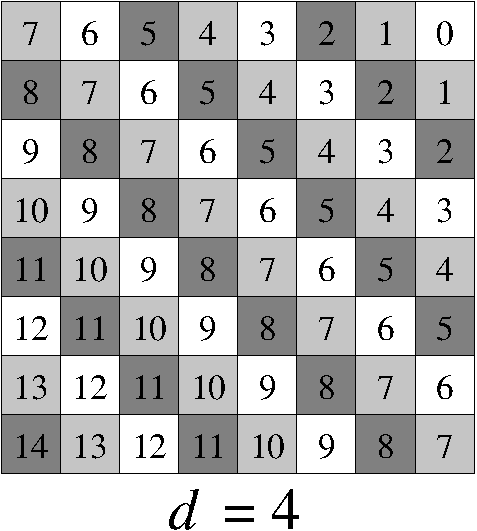
\includegraphics[width=0.23\columnwidth]{dlines4}\hspace{.5em}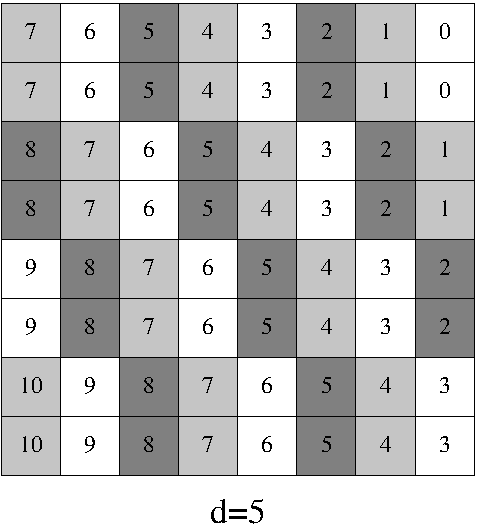
\includegraphics[width=0.23\columnwidth]{dlines5}\hspace{.5em}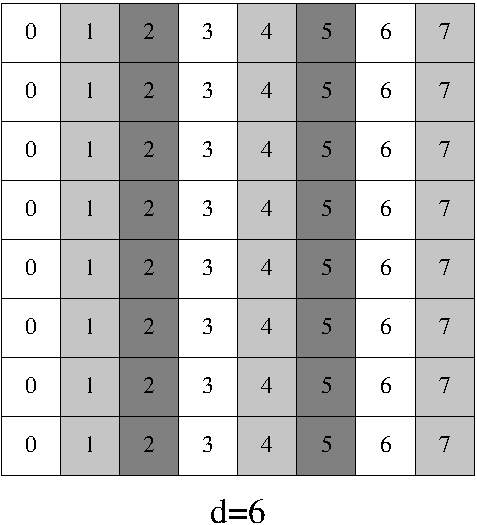
\includegraphics[width=0.23\columnwidth]{dlines6}\hspace{.5em}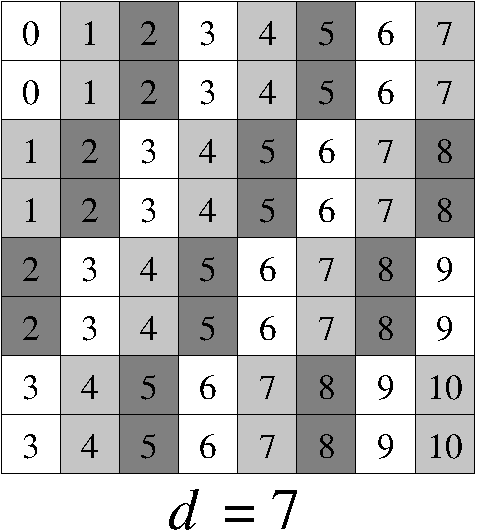
\includegraphics[width=0.23\columnwidth]{dlines7}}\caption{Line number $k$ for pixels following direction $d=0:7$ in an $8\times8$
block.\label{fig:Lines-for-direction}}
\end{figure}

For each direction $d$, the pixel average for line $k$ is determined
by:
\begin{equation}
\mu_{d,k}=\frac{1}{N_{d,k}}\sum_{p\in P_{d,k}}x_{p}\ ,\label{eq:pixel-average}
\end{equation}
where $x_{p}$ is the value of pixel $p$, $P_{d,k}$ is the set of
pixels in line $k$ following direction $d$ and $N_{d,k}$ is the
cardinality of $P_{d,k}$ (for example, in Fig.~\ref{fig:Lines-for-direction},
$N_{1,0}=2$ and $N_{1,4}=8$). The SSD is then defined as:
\begin{equation}
\sigma_{d}^{2}=\sum_{k\in\mathrm{block},d}\left[\sum_{p\in P_{d,k}}\left(x_{p}-\mu_{d,k}\right)^{2}\right]\ .\label{eq:direction-variance0}
\end{equation}

Expanding (\ref{eq:direction-variance0}) and then substituting (\ref{eq:pixel-average})
into it, we get
\begin{align}
\sigma_{d}^{2}= & \sum_{k\in\mathrm{block},d}\left[\sum_{p\in P_{d,k}}x_{p}^{2}-2\sum_{p\in P_{d,k}}x_{p}\mu_{d,k}+\sum_{p\in P_{d,k}}\mu_{d,k}^{2}\right]\nonumber \\
= & \sum_{k\in\mathrm{block},d}\left[\sum_{p\in P_{d,k}}x_{p}^{2}-2\mu_{d,k}\sum_{p\in P_{d,k}}x_{p}+N_{d,k}\mu_{d,k}^{2}\right]\nonumber \\
= & \sum_{k\in\mathrm{block},d}\left[\sum_{p\in P_{d,k}}x_{p}^{2}-\frac{1}{N_{d,k}}\left(\sum_{p\in P_{d,k}}x_{p}\right)^{2}\right]\nonumber \\
= & \sum_{p\in\mathrm{block}}x_{p}^{2}-\sum_{k\in\mathrm{block},d}\frac{1}{N_{d,k}}\left(\sum_{p\in P_{d,k}}x_{p}\right)^{2}\ .\label{eq:direction-variance1}
\end{align}
 Note that the simplifications leading to (\ref{eq:direction-variance1})
are the same as to those allowing a variance to be computed as $\sigma_{x}^{2}=\sum x^{2}-\left(\sum x\right)^{2}/N$.
Considering that the first term of (\ref{eq:direction-variance1})
is constant with respect to $d$, we simply find the optimal direction
$d_{opt}$ by maximizing the second term:
\begin{equation}
d_{opt}=\max_{d}s_{d}\,,\label{eq:direction-variance2}
\end{equation}
where 
\begin{equation}
s_{d}=\sum_{k\in\mathrm{block},d}\frac{1}{N_{d,k}}\left(\sum_{p\in P_{d,k}}x_{p}\right)^{2}\ .\label{eq:direction-variance3}
\end{equation}

We can avoid the division in (\ref{eq:direction-variance3}) by multiplying
$s_{d}$ by 840, the least common multiple of the possible $N_{d,k}$
values ($1\le N_{d,k}\le8$). When using 8\nobreakdash-bit pixel
data (for higher bit depths, we downscale to 8~bits), and centering
the values such that $-128\le x_{p}\le127$, then $840s_{d}$ and
all calculations leading to that value fit in a 32\nobreakdash-bit
signed integer.

Fig. \ref{fig:Example-of-direction} shows an example of a direction
search for an $8\times8$ block containing a line. 

\begin{figure}
\centering{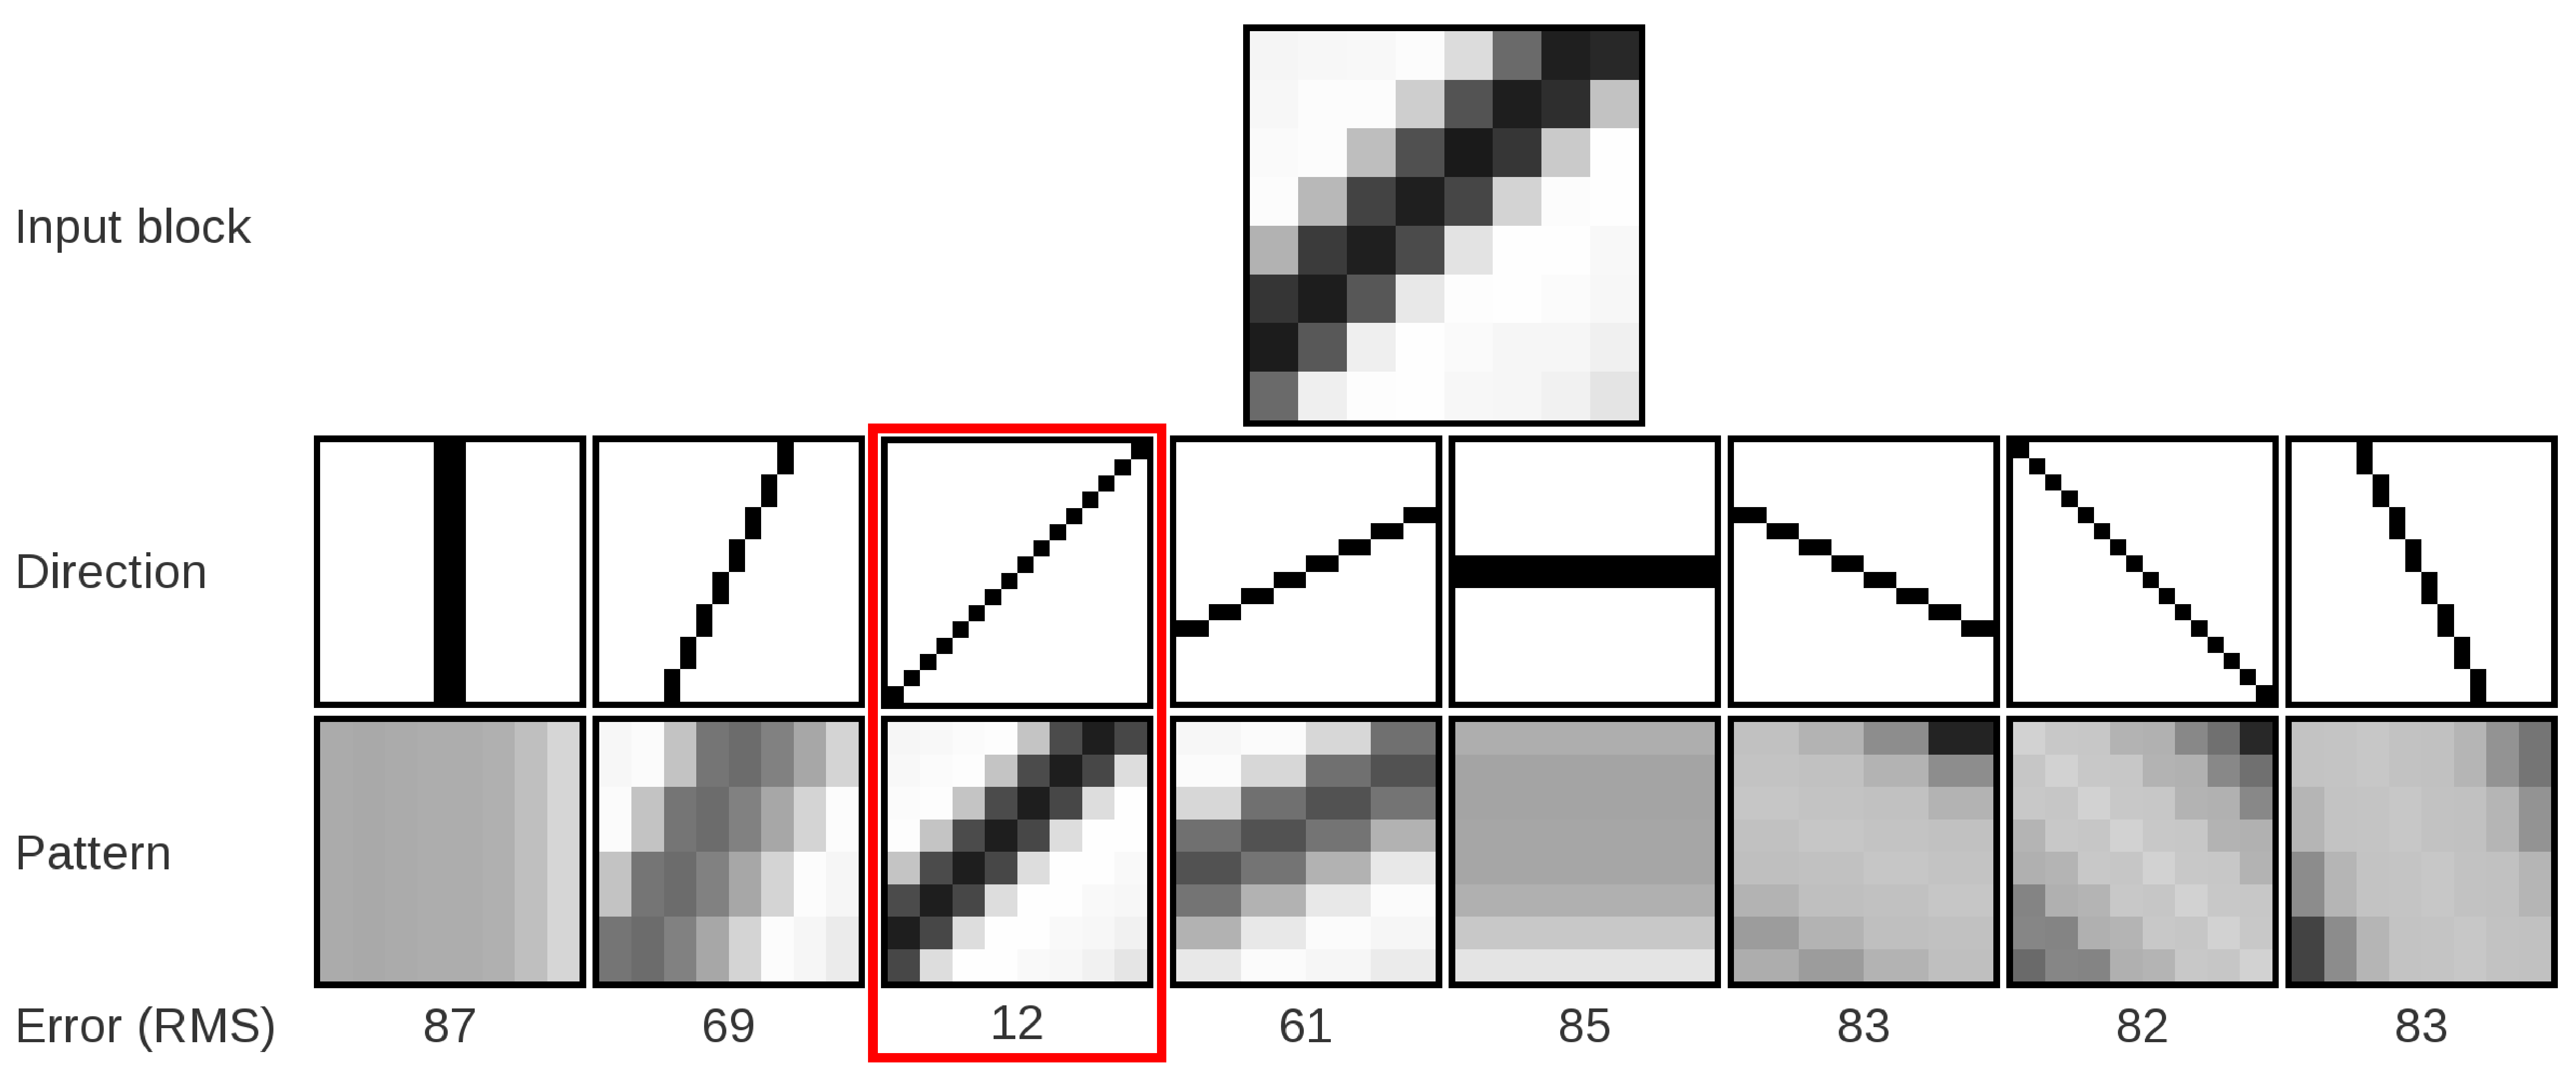
\includegraphics[width=1.0\columnwidth]{direction}}\caption{Example of direction search for an $8\times8$ block. The patterns
shown are based on the $\mu_{d,k}$ values. In this case, the 45-degree
direction is the one that minimizes $\sigma_{d}^{2}$, so it would
be selected by the search. Note that the error values $\sigma_{d}$
shown are never computed in practice (only $s_{d}$ is). \label{fig:Example-of-direction}}

\end{figure}

\newpage

\section{Non-linear Low-pass Filter}

\subsection{Detailed description}
\label{sec:nonlinear-lowpass}
The non-linear low-pass is designed to remove coding artifacts without
blurring sharp edges.  This is achieved by selecting taps based on the
identified direction and selecting filter strengths along and across
the direction independently.  The filter can be expressed as
\begin{equation}
y\left(i, j\right)=round(x(i, j) + g(\sum_{m,n \in R}w_{m,n}f(x\left(m, n) - x(i,j\right))))\label{eq:linear-filter}
\end{equation}
where $R$ contains pixels in the neighbourhood of $x(i, j)$ with the
real-valued, non-zero coefficients $w_{m,n}$, $f$ and $g$ are
non-linear functions described below, and $round(x)$ rounds $x$ to the
nearest integer (towards zero).

The function $f$ constrains the difference of the pixel to be filtered
and a neighbouring pixel.  It takes arguments the difference $d$, a
strength $S$ and a damping value $D$:
\begin{equation}
f\left(d, S, D\right)=\left\{ \begin{array}{ll}
\min\left(d, \max\left(0, S-\lfloor{\frac{d}{2^{D-\lfloor{\log_{2}S}\rfloor}}}\rfloor\right)\right) &, d>=0\\
\max\left(d, \min\left(0, \lceil{\frac{-d}{2^{D-\lfloor{\log_{2}S}\rfloor}}\rceil-S}\right)\right) &, d<0
\end{array}\right. \label{eq:constraint-function}
\end{equation}
The strength $S$ controls the maximum difference allowed minus a
ramp-down controlled by $D$.  The effect of $f$ with strengths $1$,
$2$ and $4$ and a damping value of $5$ is illustrated in
figure~\ref{fig:constraint-function}.  The function is symmetric for
$d$ values around $0$ and it can be expressed by the following pseudo
C code:
\begin{verbatim}
   sign(x) = x >= 0 ? 1 : -1
   f(d, T, D) = sign(d) * min(abs(d), max(0, T - (abs(d) >> (D - floor(log2(T))))))
\end{verbatim}
Note that \texttt{D} must be equal to or larger than \texttt{floor(log2(T))}.



\begin{figure}
\centering{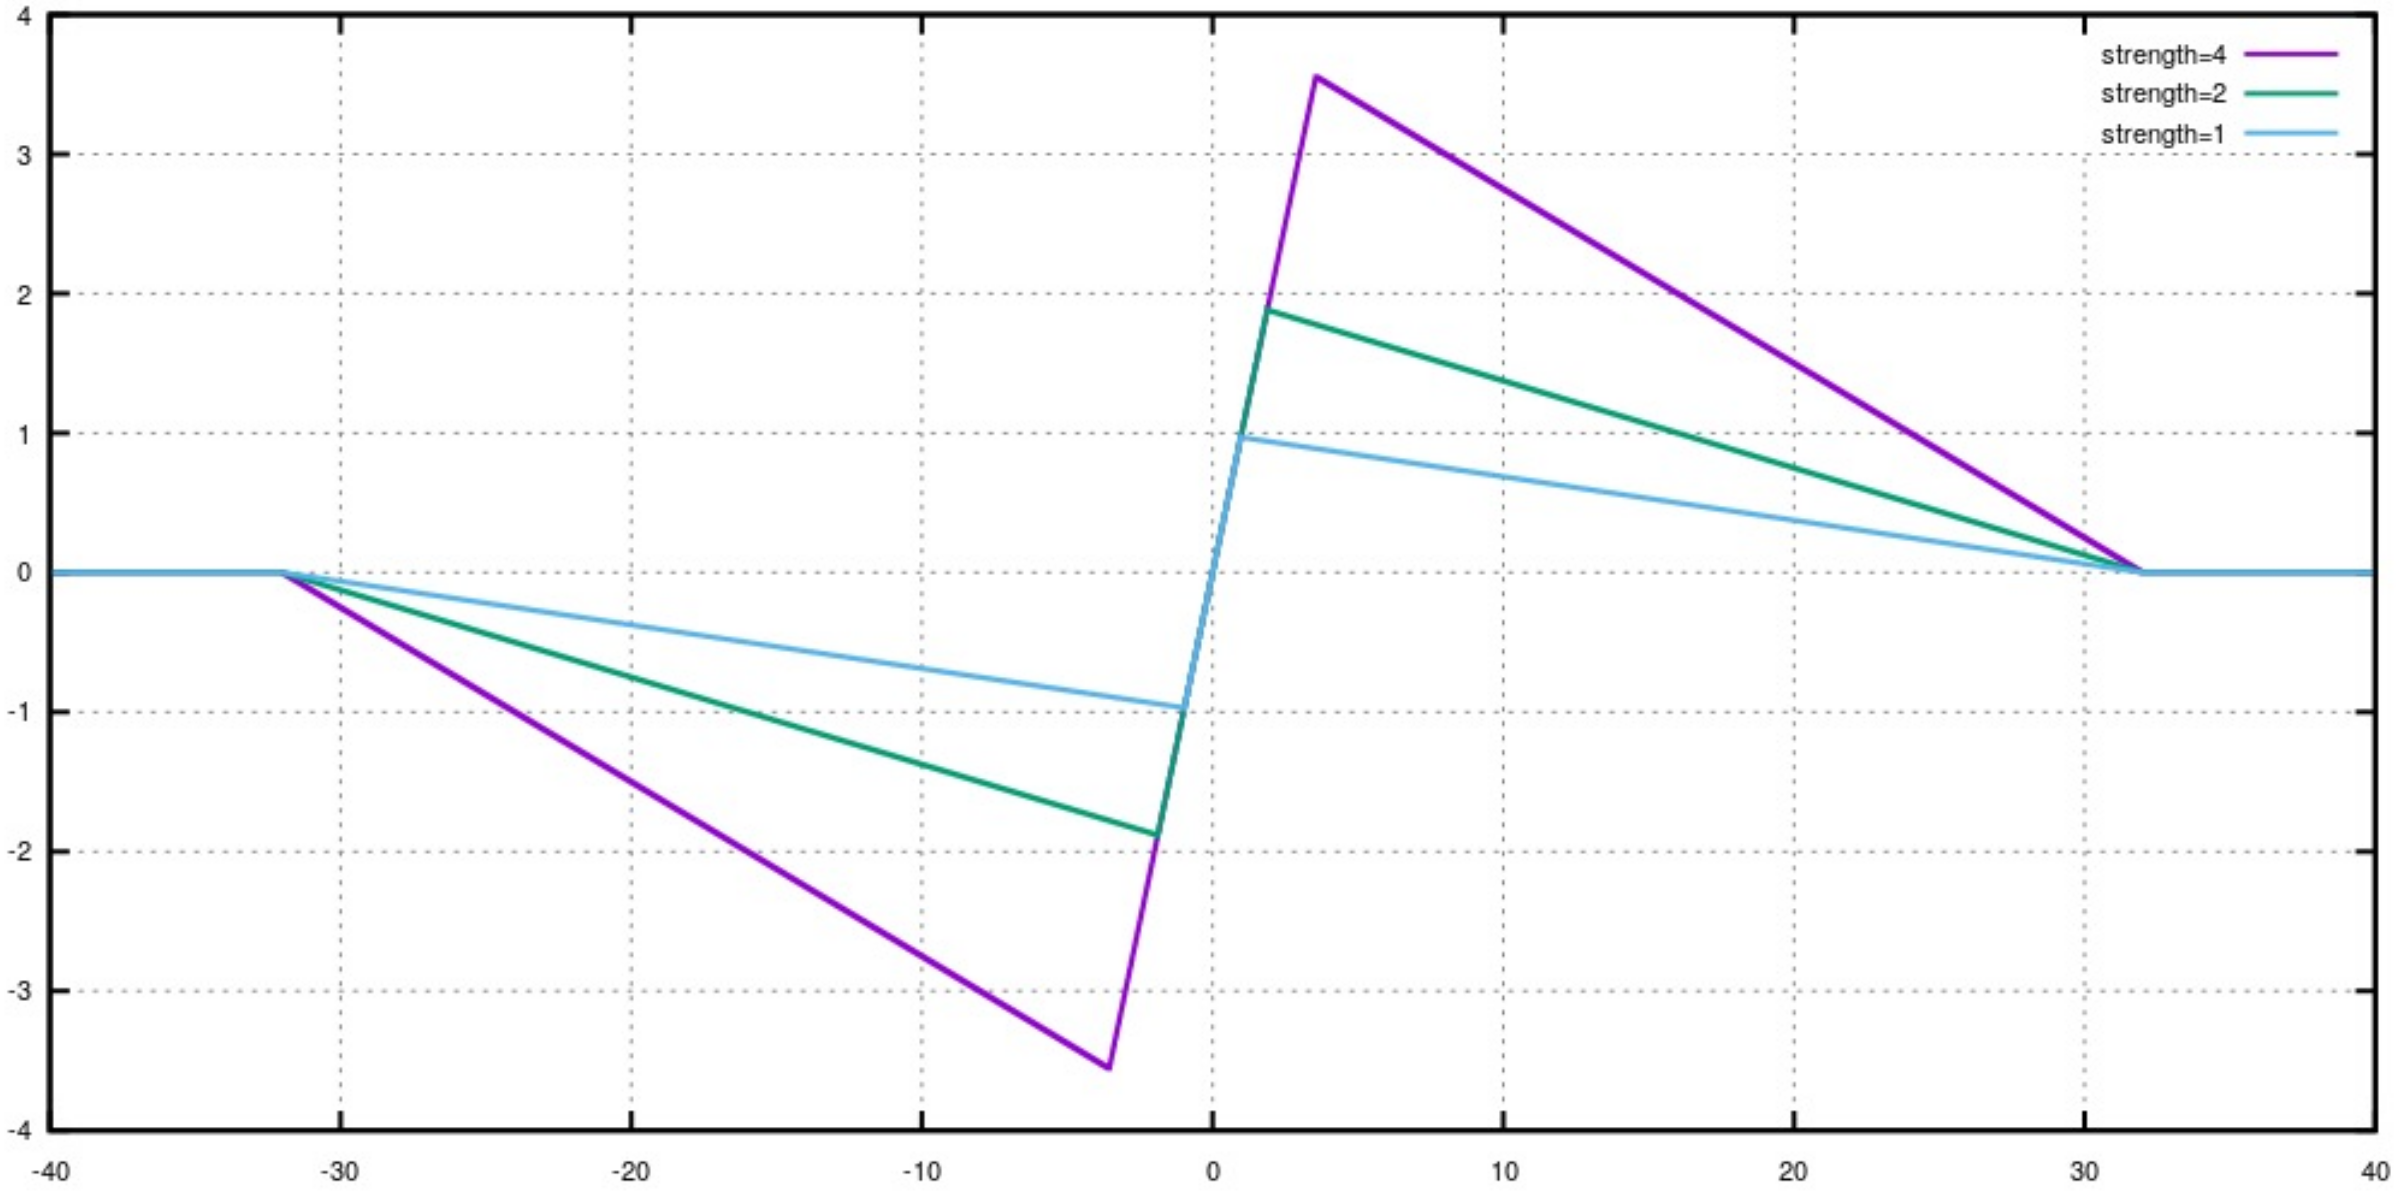
\includegraphics[width=0.9\columnwidth]{clpf_func}}

\caption{Constraint function\label{fig:constraint-function}}
\end{figure}




The function $g$ ensures that the modification $\Delta$ of the pixel
$x$ to be filtered does not exceed the greatest difference between $x$
and any $x(m,n)$:
\begin{equation}
g\left(\Delta\right)=clip\left(\Delta, \min_{m, n \in R}(x(m,n) - x(i,j), \max_{m, n \in R}(x(m,n) - x(i,j)\right)
\label{eq:cap-function}
\end{equation}
This ensures that the filtered pixel never can attain a value higher
than or lower than any of the pixels associated with the filter taps.

To allow control over the strength of the filtering along the
identified direction and the strength of the filtering across the
direction, the $S$ is allowed to differ for different
filter taps.  We therefore define \textit{primary taps} in $R'$ and
\textit{secondary taps} in $R''$ which have their associated strengths
$S'$ and $S''$ respectively.  To reflect this the filter can be expressed more specifically
as follows:
\begin{equation}
y\left(i, j\right)=round(x(i, j) + g(\sum_{m,n \in R'}{w'}_{m,n}f(x\left(m, n) - x(i,j\right), S', D) + \sum_{m,n \in R''}{w''}_{m,n}f(x\left(m, n) - x(i,j\right), S'', D)))\label{eq:linear-filter2}
\end{equation}

Both $R'$ and $R''$ depend on the direction.  $R'$ has the following
taps (the values for $w'$ are shown for their pixels relative to the filter $x$ to be filtered):



\def\arraystretch{1.5}

\begin{tabular}{XXXX}
index=0:
\noindent\begin{tabular}{|C|C|C|C|C|}
\hline
  &   &   &   &  $\frac{a}{16}$ \tabularnewline
\hline
  &      &          & $\frac{b}{16}$ &   \tabularnewline
\hline
  &      & $x$ &   &    \tabularnewline
\hline
  & $\frac{b}{16}$ &          &   &   \tabularnewline
\hline
 $\frac{a}{16}$ &   &   &   &   \tabularnewline
\hline
\end{tabular}
&
index=1:
\noindent\begin{tabular}{|C|C|C|C|C|}
\hline
  &   &     &   &   \tabularnewline
\hline
  &   &     &   & $\frac{a}{16}$  \tabularnewline
\hline
  & $\frac{b}{16}$  & $x$ & $\frac{b}{16}$  &   \tabularnewline
\hline
$\frac{a}{16}$  &   &     &   &   \tabularnewline
\hline
  &   &     &   &   \tabularnewline
\hline
\end{tabular}
&
index=2:
\noindent\begin{tabular}{|C|C|C|C|C|}
\hline
  &   &     &   &   \tabularnewline
\hline
  &   &     &   &   \tabularnewline
\hline
$\frac{a}{16}$  & $\frac{b}{16}$  & $x$ &  $\frac{b}{16}$ & $\frac{a}{16}$  \tabularnewline
\hline
  &   &     &   &   \tabularnewline
\hline
  &   &     &   &   \tabularnewline
\hline
\end{tabular}
&
index=3:
\noindent\begin{tabular}{|C|C|C|C|C|}
\hline
  &   &     &   &   \tabularnewline
\hline
$\frac{a}{16}$  &   &     &   &   \tabularnewline
\hline
  & $\frac{b}{16}$  & $x$ & $\frac{b}{16}$  &   \tabularnewline
\hline
  &   &     &   & $\frac{a}{16}$    \tabularnewline
\hline
  &   &     &   &   \tabularnewline
\hline
\end{tabular}
\tabularnewline
index=4:
\noindent\begin{tabular}{|C|C|C|C|C|}
\hline
$\frac{a}{16}$  &   &     &   &   \tabularnewline
\hline
  & $\frac{b}{16}$  &     &   &   \tabularnewline
\hline
  &   & $x$ &   &   \tabularnewline
\hline
  &   &     & $\frac{b}{16}$  &   \tabularnewline
\hline
  &   &     &   & $\frac{a}{16}$  \tabularnewline
\hline
\end{tabular}
&
index=5:
\noindent\begin{tabular}{|C|C|C|C|C|}
\hline
  & $\frac{a}{16}$  &     &   &   \tabularnewline
\hline
  &   &  $\frac{b}{16}$   &   &   \tabularnewline
\hline
  &   & $x$ &   &   \tabularnewline
\hline
  &   &  $\frac{b}{16}$   &   &   \tabularnewline
\hline
  &   &     & $\frac{a}{16}$  &   \tabularnewline
\hline
\end{tabular}
&
index=6:
\noindent\begin{tabular}{|C|C|C|C|C|}
\hline
  &   &  $\frac{a}{16}$   &   &   \tabularnewline
\hline
  &   &  $\frac{b}{16}$   &   &   \tabularnewline
\hline
  &   & $x$ &   &   \tabularnewline
\hline
  &   &  $\frac{b}{16}$   &   &   \tabularnewline
\hline
  &   &  $\frac{a}{16}$   &   &   \tabularnewline
\hline
\end{tabular}
&
index=7:
\noindent\begin{tabular}{|C|C|C|C|C|}
\hline
  &   &     & $\frac{a}{16}$  &   \tabularnewline
\hline
  &   &  $\frac{b}{16}$   &   &   \tabularnewline
\hline
  &   & $x$ &   &   \tabularnewline
\hline
  &   &  $\frac{b}{16}$   &   &   \tabularnewline
\hline
  & $\frac{a}{16}$  &     &   &   \tabularnewline
\hline
\end{tabular}
\end{tabular}

\vspace{5mm}
where $a=2$ and $b=4$ for even strengths and $a=3$ and $b=3$ for odd strengths.  $R''$ has the following taps ($w''$):

\begin{tabular}{XXXX}
index=0, 4:
\noindent\begin{tabular}{|C|C|C|C|C|}
\hline
  &   & $\frac{1}{16}$    &   &   \tabularnewline
\hline
  &   & $\frac{2}{16}$    &   &   \tabularnewline
\hline
$\frac{1}{16}$  & $\frac{2}{16}$  & $x$ & $\frac{2}{16}$  & $\frac{1}{16}$  \tabularnewline
\hline
  &   & $\frac{2}{16}$    &   &   \tabularnewline
\hline
  &   & $\frac{1}{16}$    &   &   \tabularnewline
\hline
\end{tabular}
&
index=1, 5:
\noindent\begin{tabular}{|C|C|C|C|C|}
\hline
  &   &     & $\frac{1}{16}$  &   \tabularnewline
\hline
$\frac{1}{16}$  &   &  $\frac{2}{16}$   &   &   \tabularnewline
\hline
  & $\frac{2}{16}$  & $x$ & $\frac{2}{16}$  &   \tabularnewline
\hline
  &   &  $\frac{2}{16}$   &   & $\frac{1}{16}$  \tabularnewline
\hline
  & $\frac{1}{16}$  &     &   &   \tabularnewline
\hline
\end{tabular}
&
index=2, 6:
\noindent\begin{tabular}{|C|C|C|C|C|}
\hline
$\frac{1}{16}$  &   &     &   &  $\frac{1}{16}$ \tabularnewline
\hline
  & $\frac{2}{16}$  &     & $\frac{2}{16}$  &   \tabularnewline
\hline
  &   & $x$ &   &   \tabularnewline
\hline
  & $\frac{2}{16}$  &     & $\frac{2}{16}$  &   \tabularnewline
\hline
$\frac{1}{16}$  &   &     &   & $\frac{1}{16}$  \tabularnewline
\hline
\end{tabular}
&
index=3, 7:
\noindent\begin{tabular}{|C|C|C|C|C|}
\hline
  & $\frac{1}{16}$  &     &   &   \tabularnewline
\hline
  &   &  $\frac{2}{16}$   &   & $\frac{1}{16}$  \tabularnewline
\hline
  & $\frac{2}{16}$  & $x$ & $\frac{2}{16}$  &   \tabularnewline
\hline
 $\frac{1}{16}$ &   &  $\frac{2}{16}$   &   &   \tabularnewline
\hline
  &   &     & $\frac{1}{16}$  &   \tabularnewline
\hline
\end{tabular}
\end{tabular}


\def\arraystretch{1}


\subsection{Valid strengths and damping values}

The strengths $S'$ and $S''$ and damping value $D$ must be set high
enough to smooth out coding artifacts, but low enough to avoid
blurring important details in the image.  For 8 bit content $S'$ can
have integer values between $0$ and $15$, and $S''$ can be $0$, $1$,
$2$ or $4$.  $D$ can be set to $3$, $4$, $5$ or $6$ for luma, and the
damping value for chroma is always one less.  The damping value shall
never be lower than the $log_2$ of the strength to ensure that
$2^{D-\lfloor{\log_{2}S}\rfloor}$ in the constraint function never
becomes less than $1$.  For instance, if the chroma $S'$ is $15$ and the luma damping is $3$,
the chroma damping shall also be $3$ because $log_2(S')$ is $3$.

For content above 8 bit, $S'$ and $S''$ must be scaled according to
the extra bit depth, and $D$ offset corresponingly, so for 12 bit
content $S'$ can have the values $0$, $16$, $32$, $...$, $240$, and
$D$ can have the values $7$, $8$, $9$ and $10$.  Picking an optimial
damping value is less critical for compression gains than picking the
optimal strengths.  $S'$ and $S''$ are are set independently for
luma and chroma.

\section{Signaling and Superblocks}

Some CDEF parameters are signaled at the frame level, and some
parameters may be signaled at the superblock level.  The following is
signaled at the frame level: the damping $D$ (2 bit), the number of
bits used for superblock signaling (0-3, 2 bits), and a list of 1, 2,
4, 8 or 16 presets.  One preset contains the luma primary strength (4
bits), the chroma primary strength (4 bits), the luma secondary
strength (2 bits), the chroma secondary strength, a luma skip
condition bit, and a chroma skip condition bit (a total of 14 bits per
preset).

The filtering is applied one superblock at a time.  For each
superblock, the 0 - 3 bits are read to indicate the preset that will
be used for this superblock.  On inter-predicted frames, the filter
parameters are only coded for superblocks that are not completely
skipped.  Superblocks where no level is coded have CDEF disabled.
Similarly, any skipped coding block within a superblock has filtering
disabled if the skip condition bit is not set.

When the pixels used for a filter lie outside of the viewable image,
we set $f\left(d,S,D\right)=0$ in equation~\ref{eq:constraint-function}.

Since the skip condition flag would be redundant in the case when both
the primary and secondary filter strengths are $0$, this combination
has a special meaning.  If the skip condition flag is set and both the
primary and secondary strengths have been signaled as $0$, then the
block shall be filtered with a primary filter strength equal to $19$
and a secondary filter strength equal to $7$.  The skip condition
flag is still to be regarded as $1$.

If the chroma subsampling differs horizontally and vertically,
e.g. 4:2:2 video, the filter is disabled for chroma, and the chroma
primary strength, the chroma skip condition flag and the chroma
secondary strength are not signaled.

The bitstream syntax is summarized in tables~\ref{header_syntax}, \ref{params_syntax} and \ref{partition_syntax}.

\begin{table}[]
\centering
\caption{Uncompressed header syntax}
\label{header_syntax}
\begin{tabular}{|l|l|}
\hline
... &  \\ \hline
loop\_filter\_params( ) &  \\ \hline
\textcolor{red}{cdef\_params()} &  \\ \hline
quantization\_params( ) &  \\ \hline
... &  \\ \hline
\end{tabular}
\end{table}

\begin{table}[]
\centering
\caption{CDEF params syntax}
\label{params_syntax}
\begin{tabular}{|l|l|}
\hline
\textcolor{red}{cdef\_params()} \{ &  \\ \hline
\enspace \textcolor{red}{damping} & \textcolor{red}{f(2)} \\ \hline
\enspace \textcolor{red}{cdef\_bits} & \textcolor{red}{f(2)} \\ \hline
\enspace \textcolor{red}{for (cdef\_id = 0; cdef\_id < 1 <{<} cdef\_bits; cdef\_id++) \{} &  \\ \hline
\quad \textcolor{red}{cdef\_luma\_primary\_strength[cdef\_id]} & \textcolor{red}{f(4)} \\ \hline
\quad \textcolor{red}{cdef\_luma\_skip\_condition[cdef\_id]} & \textcolor{red}{f(1)} \\ \hline
\quad \textcolor{red}{cdef\_luma\_secondary\_strength[cdef\_id]} & \textcolor{red}{f(2)} \\ \hline
\quad \textcolor{red}{if (subsampling\_x == subsampling\_y) \{} & \\ \hline
\enspace \quad \textcolor{red}{cdef\_chroma\_primary\_strength[cdef\_id]} & \textcolor{red}{f(4)} \\ \hline
\enspace \quad \textcolor{red}{cdef\_chroma\_skip\_condition[cdef\_id]} & \textcolor{red}{f(1)} \\ \hline
\enspace \quad \textcolor{red}{cdef\_chroma\_secondary\_strength[cdef\_id]} & \textcolor{red}{f(2)} \\ \hline
\quad \textcolor{red}{\}} & \\ \hline
\enspace \textcolor{red}{\}} & \\ \hline
\textcolor{red}{\}} &  \\ \hline
\end{tabular}
\end{table}

\begin{table}[]
\centering
\caption{Decode partition syntax}
\label{partition_syntax}
\begin{tabular}{|l|l|}
\hline
... &  \\ \hline
if (bsize == BLOCK\_8X8 || partition != PARTITION\_SPLIT) \{ &  \\ \hline
\enspace for (i = 0; i < num8x8; i++) \{ &  \\ \hline
\quad AbovePartitionContext[c + i] = 15 >{>} b\_width\_log2\_lookup[subsize] &  \\ \hline
\quad LeftPartitionContext[r + i] = 15 >{>} b\_height\_log2\_lookup[subsize] &  \\ \hline
\enspace \} &  \\ \hline
\} &  \\ \hline
\textcolor{red}{if (bsize == BLOCK\_64X64) \{} & \\ \hline
\enspace \textcolor{red}{if (!sb\_all\_skip(MiCol, MiRow, 64 / MI\_SIZE)) \{} & \\ \hline
\quad \textcolor{red}{cdef\_id } & \textcolor{red}{f(cdef\_bits)} \\ \hline
\enspace \textcolor{red}{\}} & \\ \hline
\textcolor{red}{\}} & \\ \hline
... &  \\ \hline
\end{tabular}
\end{table}

\section{Superblock Decode Process}

For each 8x8 block within a superblock, the following steps are applied.

\subsection{Direction Search}

The direction search evaluates equation (\ref{eq:direction-variance3})
for each of the 8 directions, with the $\frac{1}{N_{d,k}}$ factor
being replaced by an exact 10-bit multiply by $\frac{840}{N_{d,k}}$. The step-by-step process is
described in algorithm~\ref{cap:direction-search}.  The search is only
done for the luma component, and the direction found in this search
will be used for all components.

In total, the search for all 8 directions requires the following
arithmetic operations:
\begin{enumerate}
\item The pixel accumulations in equation (\ref{eq:direction-variance3})
are 418 adds of 8-bit signed values, with results that fit in 11 bits.
There's a maximum of 8 values contributing to each sums (there are
simplifications that can save 128 adds using intermediate sums).
\item The result of 1) is 90 11-bit partial sums. Each is squared (so 90
11-bit multiplies), with the result being 21-bit unsigned values.
Each of these is multiplied by one of eight different 10-bit constants,
with the result guaranteed to fit in 27 bits. Since some lines use
the same constant and are eventually added together, only 34 multiplies
by constants are needed after simplification. 
\item There are another 86 adds from the results of step 2), resulting in
8 29-bit unsigned values. There's a maximum of 15 values contributing
to each of these sums.
\item The resulting values in 3) are compared to find the largest value. 
\end{enumerate}

\begin{algorithm}[t]
\noindent\fbox{%
\begin{varwidth}{\dimexpr\linewidth-2\fboxsep-2\fboxrule\relax}
\begin{algorithmic}
\STATE {Initialize all variables to zero}
\FOR{$d=0$ to $7$}
  \FOR{$i=0$ to $7$}
    \FOR{$j=0$ to $7$}
      \STATE $L \leftarrow \textrm{line\_table}[d][i][j]$
      \STATE $\textrm{partial}[d][L] \leftarrow \textrm{partial}[d][L] + \lfloor{\textrm{pixel}[i][j] \cdot 2^{8 - \textrm{bitdepth}}\rfloor - 128}$
      \STATE $\textrm{count}[d][L] \leftarrow \textrm{count}[d][L] + 1$
    \ENDFOR
  \ENDFOR
  \FOR{$L=0$ to $14$}
    \IF{$\textrm{count}[d][L] > 0$}
      \STATE $s[d] \leftarrow s[d] + \textrm{partial}[d][L]^2\cdot 840/\textrm{count}[d][L]$
    \ENDIF
  \ENDFOR
\ENDFOR
\FOR{$d=0$ to $7$}
  \IF{$s[d] > s[\textrm{best\_}d]$}
    \STATE $\textrm{best\_}d \leftarrow d$ 
  \ENDIF
\ENDFOR
\STATE $\textrm{direction} \leftarrow \textrm{best\_}d$
\STATE $\textrm{variance} \leftarrow s[\textrm{best\_}d] - s[(\textrm{best\_}d+4) \mod 8]$
\end{algorithmic}
\end{varwidth}% 
}

\caption{Direction search. The line\_table[$d$][$i$][$j$] values are the line numbers shown
in Fig.~\ref{fig:Lines-for-direction}. Note that in a practical implementation,
the $840/\textrm{count}[d][L]$ term does not need to be computed, since it
only depends on $d$ and $L$\label{cap:direction-search}.}
\end{algorithm}

\subsection{Strength Computation}

The signaled primary strength $S'$ is adjusted for luma using a
variance $v$ (see algorithm~\ref{cap:direction-search}) for the 8x8 block as follows:
\begin{equation}
{S'}_{adj}=\left\{ \begin{array}{ll}
\lfloor\frac{S' (4 + \min(\lfloor log_2\lfloor\frac{v}{2^{16}}\rfloor \rfloor, 12)) + 8}{16}\rfloor &, v >= 2^{10}\\
0 &, otherwise
\end{array}\right. \label{eq:strength-adjustment}
\end{equation}

This adjustment is not applied for chroma, nor for the secondary strength $S''$.

\subsection{Directional Filtering}

For each 8x8 block to be filtered, the directional filter is applied
in a single pass using the strengths ${S'}_{adj}$ and ${S''}$ for luma
or ${S'}$ and ${S''}$ for chroma, and damping value $D$. When
filtering pixel $(i,j)$, the directional filter may use pixels that
are outside of the 8x8 block, or even outside of the superblock. If
the input pixel lies outside of the frame, then the pixel is ignored,
i.e. $f(d,S,D)=0$. The filter and weights for each direction $d$ are
described in Section~\ref{sec:nonlinear-lowpass}.  Note that in some
cases (when the direction index value is odd) some taps in $R'$ and
$R''$ have the same positions, but their weigths in
$R'$ and $R''$ are separate.


\section{Results}

We tested the deringing filter using the Are We Compressed
Yet~\cite{AWCY} online testing tool. The results are shown in
table~\ref{tab:bd-rate} for the objective-1-fast test set.  These
results reflect the gains in the codebase for git SHA \texttt{e200b28}
(8th August 2017).

\begin{table}
\caption{CDEF Bjontegaard-delta~\cite{Testing-draft} rate for
the objective-1-fast test set in AWCY.\label{tab:bd-rate}}
\centering{%
\begin{tabular}{cccccc}
\hline 
Bitrate (bpp) & PSNR & CIEDE 2000 & PSNR-HVS & SSIM & MS-SSIM\tabularnewline
\hline 
High-latency & -1.08\% & -2.11\% & -0.15\% & -1.11\% & -0.44\%\tabularnewline
Low-latency & -1.93\% & -2.88\% & -0.86\% & -1.96\% & -1.18\%\tabularnewline
Low-latency, cpu-used=4 & -3.68\% & -4.54\% & -2.50\% & -4.15\% & -3.05\%\tabularnewline
\hline 
\end{tabular}}

\end{table}

CDEF competes for the same gains as some other coding tools, in
particular the dual\_filter tool and to a lesser degree motion\_var
and ext\_tx.  Disabling these tools roughly doubles the CDEF gains.
In medium to low complexity configurations excluding one or more of
these tools while keeping CDEF enabled may give a better
compexity/compression trade-off.

Subjective tests have shown a significant
improvement in quality~\cite{AV1-CLPFVSCDEF} over CLPF which was
proposed in the early stages of AV1 development~\cite{AV1-CLPF}.


\section{Conclusion}

We have demonstrated an effective algorithm for removing coding
artifacts from coded images and videos. By taking into account the
direction of the patterns, the risk of blurring is reduced. Objective
results show a bit-rate reductions up to 20\% depending on the encoder
configuration and video content.

\bibliographystyle{IEEEtran}
\bibliography{daala}

\end{document}
